\documentclass[tikz,border=2pt]{standalone}
\usepackage{amsmath,amssymb}
\usepackage{tikz}
\usetikzlibrary{arrows.meta,matrix}

\begin{document}
% The three elementary row operations, each reversible, so they never change the solution set.
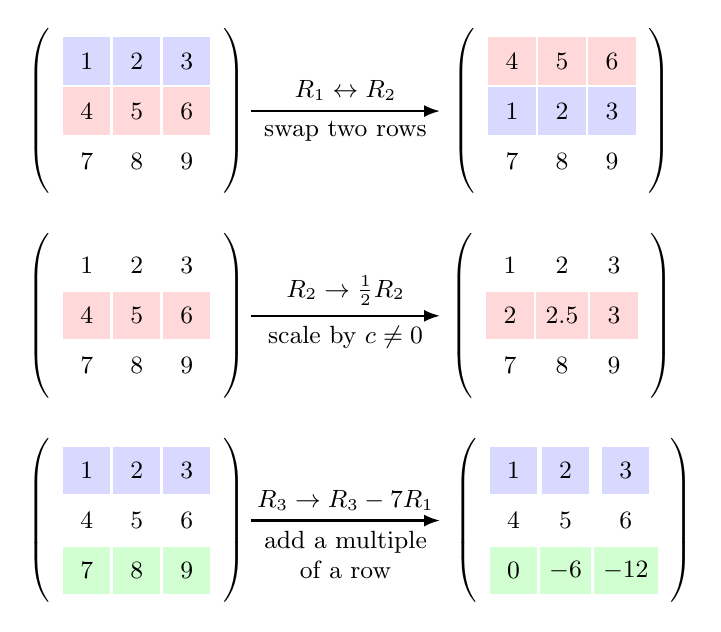
\begin{tikzpicture}[every node/.style={font=\small}, >={Latex[length=2mm]}, m/.style={matrix of math nodes, nodes={minimum size=6mm, anchor=center}, left delimiter=(, right delimiter=), column sep=1pt, row sep=1pt}]
	\matrix (A) [m] at (0,0) {
		|[fill=blue!15]| 1 & |[fill=blue!15]| 2 & |[fill=blue!15]| 3 \\
		|[fill=red!15]| 4 & |[fill=red!15]| 5 & |[fill=red!15]| 6 \\
		7 & 8 & 9 \\
	};
	\draw[->, thick] (1.45,0) -- (3.85,0) node[midway, above, font=\small] {$R_1\leftrightarrow R_2$} node[midway, below, font=\small] {swap two rows};
	\matrix (B) [m] at (5.4,0) {
		|[fill=red!15]| 4 & |[fill=red!15]| 5 & |[fill=red!15]| 6 \\
		|[fill=blue!15]| 1 & |[fill=blue!15]| 2 & |[fill=blue!15]| 3 \\
		7 & 8 & 9 \\
	};
	\begin{scope}[yshift=-2.6cm]
		\matrix (C) [m] at (0,0) {
			1 & 2 & 3 \\
			|[fill=red!15]| 4 & |[fill=red!15]| 5 & |[fill=red!15]| 6 \\
			7 & 8 & 9 \\
		};
		\draw[->, thick] (1.45,0) -- (3.85,0) node[midway, above, font=\small] {$R_2\to\tfrac12R_2$} node[midway, below, font=\small] {scale by $c\neq0$};
		\matrix (D) [m] at (5.4,0) {
			1 & 2 & 3 \\
			|[fill=red!15]| 2 & |[fill=red!15]| 2.5 & |[fill=red!15]| 3 \\
			7 & 8 & 9 \\
		};
	\end{scope}
	\begin{scope}[yshift=-5.2cm]
		\matrix (E) [m] at (0,0) {
			|[fill=blue!15]| 1 & |[fill=blue!15]| 2 & |[fill=blue!15]| 3 \\
			4 & 5 & 6 \\
			|[fill=green!18]| 7 & |[fill=green!18]| 8 & |[fill=green!18]| 9 \\
		};
		\draw[->, thick] (1.45,0) -- (3.85,0) node[midway, above, font=\small] {$R_3\to R_3-7R_1$} node[midway, below, font=\small, align=center] {add a multiple\\ of a row};
		\matrix (F) [m] at (5.55,0) {
			|[fill=blue!15]| 1 & |[fill=blue!15]| 2 & |[fill=blue!15]| 3 \\
			4 & 5 & 6 \\
			|[fill=green!18]| 0 & |[fill=green!18]| -6 & |[fill=green!18]| -12 \\
		};
	\end{scope}
\end{tikzpicture}
\end{document}
